\section{Time convergence and mesh independence study}

\begin{itemize}
    \item How do I compute the closure terms with the average methodo (Mehrabahdi)
    \item Mesh and size independence study 
    \begin{itemize}
        \item Rising velocity
        \item Velocity fluctuation / Reynolds stress convergence 
        \item PFP time convergence
    \end{itemize}
    \item Loisy single rising drop
    \item Show that eulerian two-point correlation does indeed decay in a tri periodic domain 
\end{itemize}

\subsubsection{Fixed array of bubbles}

\begin{figure}[h!]
    \centering
    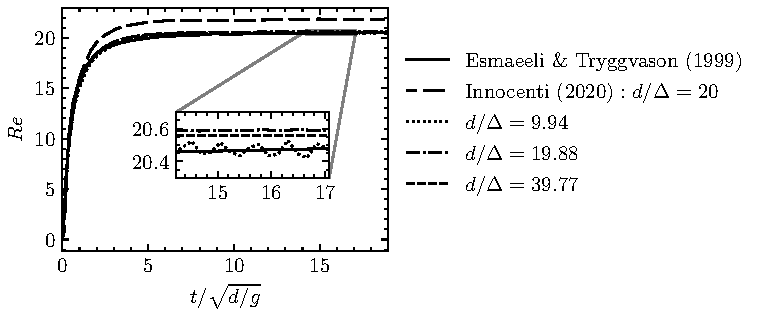
\includegraphics[height = 0.3\textwidth]{image/VALIDATION2.0/Loisy/Re.pdf}
    \caption{Time evolution of the Reynolds number based on the drift velocity $U = \avg{\textbf{u}}_d - \avg{\textbf{u}}$ with $\phi = 0.1256$ ,$\rho_r =\mu_r =10$ and $Ga = 29.9$.}
\end{figure}


\subsubsection{Free array of droplets}



The first plot concerns the continuous averaged quantities
\begin{figure}[h!]
    \centering
    % 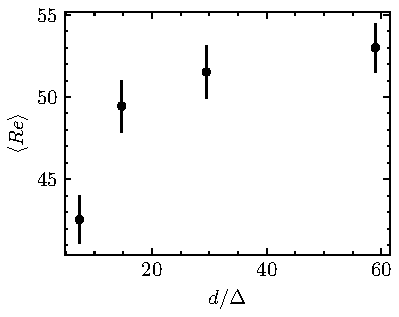
\includegraphics[height = 0.3\textwidth]{image/VALIDATION2.0/fCA/Re.pdf}
    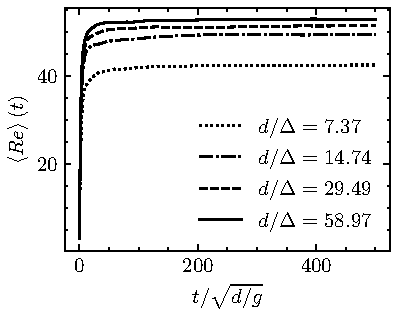
\includegraphics[height = 0.3\textwidth]{image/VALIDATION2.0/fCA/Recum.pdf}
    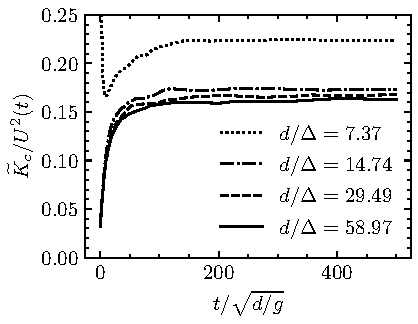
\includegraphics[height = 0.3\textwidth]{image/VALIDATION2.0/fCA/Tcum.pdf}
    \caption{(left) Cumulative mean of the volume averaged Reynolds number along the simulation time based on the drift velocity $U = \avg{\textbf{u}}_d - \avg{\textbf{u}}_c$, with $\phi = 0.1$, $\rho_r = 1.11$, $ \mu_r =0.1$ and $Ga = 29.9$ and $N_b = 125$.
    (right) Cumulative mean of the fluid Reynolds stress tesor. }
\end{figure}

This second plot focus on the particular averaged quantities : 
\begin{figure}[h!]
    \centering
    % 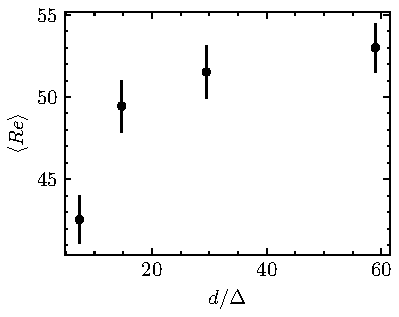
\includegraphics[height = 0.3\textwidth]{image/VALIDATION2.0/fCA/Re.pdf}
    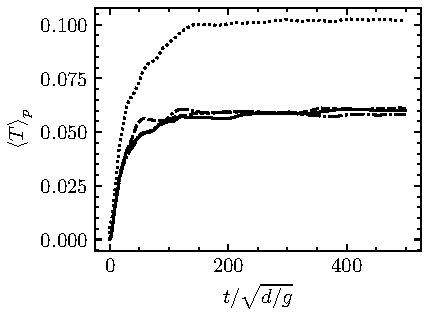
\includegraphics[height = 0.3\textwidth]{image/VALIDATION2.0/fPA/Tcum.pdf}
    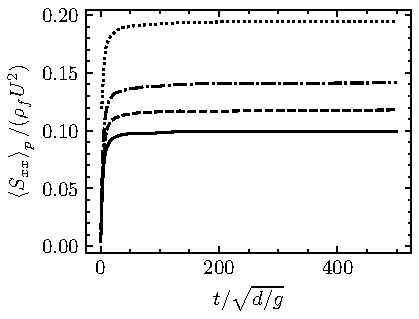
\includegraphics[height = 0.3\textwidth]{image/VALIDATION2.0/fPA/Scum.pdf}
    \caption{(left) Cumulative mean of the volume averaged granular temperature along the simulation time based on the drift velocity $U = \avg{\textbf{u}}_d - \avg{\textbf{u}}_c$, with $\phi = 0.1$, $\rho_r = 1.11$, $ \mu_r =0.1$ and $Ga = 29.9$ and $N_b = 125$.
    (right) Cumulative mean of the dimensionless particle-fluid-particle stress horizontal component tensor. }
\end{figure}
\begin{figure}[h!]
    \centering
    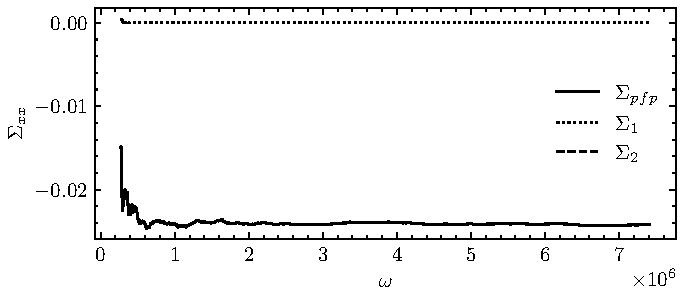
\includegraphics[height = 0.3cm]{image/VALIDATION2.0/fPA/PFPxx_x3.pdf}
    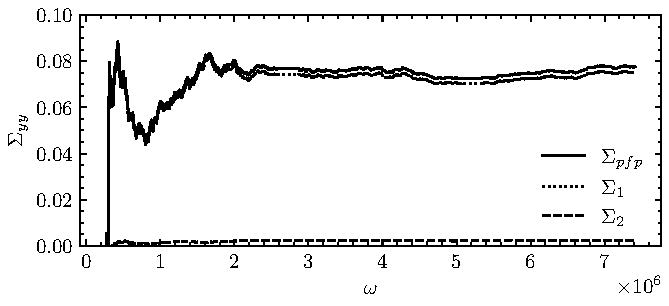
\includegraphics[height = 0.3cm]{image/VALIDATION2.0/fPA/PFPyy_x3.pdf}
    \caption{
    (right) Cumulative mean of the dimensionless particle-fluid-particle stress horizontal component tensor decomposed into $\Sigma_{pfp}= \Sigma_1+\Sigma_2$ in terms of the number of realization $\omega$. }
\end{figure}
